
\section{$N$-particle Systems}
\label{sec:n-particle-systems}

Generally a system of $N$ particles can be described by a system of
$6N$ Hamiltonian equations, however, in most systems the size of $N$
is so large that it rapidly becomes impractical to solve such a system
of equations to determine the behaviour of the system, and so at least
one of a number of approaches must be taken to simplify the analysis.

\begin{description}
\item[Test Particles] This is an exact solution for some $M \ll N$
  particles of the system, while the rest are treated as an external
  slowly evolving medium.
\item[Hydrodynamic Descriptions of Plasma] We assume a plasma to be
  continuous at a scale much greater than the mean free path of
  particles within the material.
\item[Classical Kinetics] studies the relationship between motion and
  the forces affecting the motion using statistical methods.
\end{description}

In fluid dynamics the motion of fluids is studied on a macroscopic
scale, with the fluid regarded as a continuous medium. The fluid is
described by macroscopic parameters, such as fluid density, fluid
velocity, and pressure.

\section{Deriving the Hydrodynamic Equations}
\label{sec:deriv-hydr-equat}

\subsection{Conservation of Matter}
\label{sec:conservation-matter}
%\begin{derivation}
  Consider a fluid with a mass density $\rho$, and a volume $V$. The
  mass of the fluid is then
  \begin{equation}
    \label{eq:1}
    m = \int_V \rho \dd{V}
  \end{equation}
\marginpar{
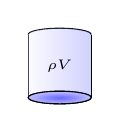
\begin{tikzpicture}[scale=0.4]
    \draw (1,0) arc (180:360:1cm and 0.2cm);
    \draw (1,0) arc (180:0:1cm and 0.2cm);
    \draw (1,2) arc (180:0:1cm and 0.2cm);
	\draw (1,0) -- (1,2); \draw (3,0) -- (3,2);
    \shade[left color=blue!5!white,right color=blue!60!white,opacity=0.3] (1,0) arc (180:360:1cm and -0.2cm) -- (3,0) -- (3,2) arc (180:360:-1cm and -0.2cm) -- (1,2) -- cycle; 
    \shade[draw=black,shading=radial, outer color=blue!25!white,inner color=blue!60!white,opacity=1] (2,0) circle (1cm and 0.2cm);
    \draw (2,1) node {\tiny $\rho V$};
\end{tikzpicture}
}
  Let $\dd{s}$ be a surface element of the volume, then the matter flux
  through that surface is $\rho\ \vec{v}\ \dotproduct \dd{\vec{s}}$, with
  a positive flux representing eflux, and a negative flux
  influx. Assuming there are no sources or sinks inside the volume $V$
  then the total mass of fluid flowing out of the volume $V$ per unit
  time is
  \begin{equation}
    \label{eq:2}
    \dv{m}{t} = \oint_{\partial V} \rho \ \vec{v}\ \dotproduct \dd{\vec{s}} 
    = - \pdv{t} \int_V \rho  \dd{V}
  \end{equation}
\marginpar{
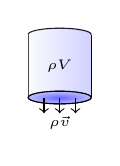
\begin{tikzpicture}[scale=0.4]
    \draw (1,0) arc (180:360:1cm and 0.2cm);
    \draw (1,0) arc (180:0:1cm and 0.2cm);
    \draw (1,2) arc (180:0:1cm and 0.2cm);
	\draw (1,0) -- (1,2); \draw (3,0) -- (3,2);
    \shade[left color=blue!5!white,right color=blue!60!white,opacity=0.3] (1,0) arc (180:360:1cm and -0.2cm) -- (3,0) -- (3,2) arc (180:360:-1cm and -0.2cm) -- (1,2) -- cycle; 
    \shade[draw=black,shading=radial, outer color=blue!25!white,inner color=blue!60!white,opacity=1] (2,0) circle (1cm and 0.2cm);

	\foreach \x in {0.5, 1, ..., 1.75} {
		\draw [<-] (1+\x, -0.5) -- (1+\x, 0);
	}
	\draw (2, -0.8) node {\tiny $\rho\vec{v}$};
	\draw (2,1) node {\tiny $\rho V$};
\end{tikzpicture}
}
  As long as the mass in the volume $V$ is conserved the two expressions
  for the mass, equations (\ref{eq:1}) and (\ref{eq:2}) can be equated.
  \begin{equation}
    \label{eq:3}
    \pdv{t} \int_V \rho \dd{V} = \oint_{\partial V} \rho \ \vec{v}\ \dotproduct \dd{\vec{s}}
  \end{equation}
  Then, applying Green's Theorem,
  \begin{equation*}
    \label{eq:4}
    \oint_{\partial V} \rho \ \vec{v} \vdot \dd{\vec{s}} = \int_V \nabla(\rho \vec{v}) \dd{V}
  \end{equation*}
  so
  \begin{equation}
    \label{eq:5}
    \oint_{\partial V} \qty( \pdv{\rho}{t} + \nabla \vdot (\rho \vec{v}) ) \dd{V} = 0
  \end{equation}
  This must be true for any volume, so we can remove the integral,
  leaving the continuity equation.
%\end{derivation}

\begin{fequation}[Fluid Continuity Equation]
\label{eq:continuity}
\newcommand{\EQcontinuity}{
   \pdv{\rho}{t} + \rho \ \nabla \vdot \vec{v} + \vec{v} \vdot \nabla \rho = 0
}
   \EQcontinuity
\end{fequation}




% \newcommand{\pdim}[1]{\scriptstyle{\mathsf{#1}} }
% \newcommand{\DIMmass}[1][\ ]{\pdim{M}^{#1}}
% \newcommand{\DIMlength}[1][\ ]{\pdim{L}^{#1}}
% \newcommand{\DIMtime}[1][\ ]{\pdim{T}^{#1}}
% \newcommand{\DIMmassdensity}{
% \DIMmass \DIMlength[-3]
% }
% \newcommand{\DIMvelocity}{
% \DIMlength \DIMtime[-1]
% }

% \begin{tabularx}{0.95\linewidth}{ccX} 
%   Symbol    & Dimensions        & Description  \\
%   \hline \hline
%   $\rho$    & $\DIMmassdensity$ & mass density \\
%   $\vec{v}$ & $\DIMvelocity$    & velocity \\
% \end{tabularx}

We can also define a current density,
\begin{equation}
  \label{eq:6}
  \vec{\jmath} = \rho \vec{v}
\end{equation}
as the \emph{mass flux density}.

\subsection{Equations of Motion}
\label{sec:equations-motion}

The equations of motion of the system can be found by considering the
conservation of momentum in the system. Consider some volume in a
fluid, then the total force acting on this volume is equal to the
integral of the pressure,
\begin{equation}
  \label{eq:7}
  F = - \oint_{\partial V} p \dd{\vec{s}}
\end{equation}
with $p(\vec{r}(t), t)$ the pressure, and the integral taken over the
boundary of the volume. Thus
\begin{equation}
  \label{eq:8}
  - \oint_{\partial V} p \dd{\vec{s}} = - \int_V \nabla p \dd{V}
\end{equation}
That is, we are saying that the force $- \nabla p$ acts on a unit
volume of the fluid. The equation of motion of a volume element in the
fluid, using Newton's second law, is
\begin{equation}
  \label{eq:9}
  \rho \dv{\vec{v}}{t} = - \nabla p
\end{equation}
where $\dv{\vec{v}}{t}$ is the rate of change in velocity of a fluid
element, and not of the fluid at that point.

\subsubsection{The Lagrangian and Eulerian Descriptions}
\label{sec:lagr-euler-descr}

By following the elements of the fluid along its flow we have a
Lagrangian fluid element, much like following a boat along a river,
and so we label each element in the fluid, and as a result the
coordinate system moves over time. The derivative of any given
function in the fluid is the convective derivative. The flow is then
described by a function $X(a, t)$, giving the position of a fluid
element labelled $a$ at time $t$.

By describing the properties of the fluid at each fixed position we
reach the Eulerian description. Here the flow is described by the
function $v(x,t)$, giving the velocity of the fluid at a point $(x,t)$
in spacetime.

These two solutions can be related. Consider a function $f(t,
\vec{r}(t))$ of a fixed Langrangian fluid element. The derivative of
$f$ with respect to time $t$ can be written
\begin{equation}
  \label{eq:10}
  \dv{f}{t} = \pdv{f}{t} + \pdv{f}{\vec{r}} \dv{\vec{r}}{t} 
            = \pdv{f}{t} + \vec{v} \pdv{f}{\vec{r}}
\end{equation}

We can define an operator, $\adv{t}$, the convective derivative,
\begin{definition}[Convective Derivative]
  \[ \adv{t} = \pdv{t} + \vec{v} \vdot \nabla \]
\end{definition}
which describes the change of a function as experienced by a specific
flow parcel.
\begin{example}[Driving in the rain]
  Say you are driving through a rainstorm, where the amount of
  rainfall is described by a function of the form $R(x,t)$ (so perhaps
  the volume of rain falling at any given point per unit of time),
  then in order to understand how conditions change as you drive along
  you must consider the rate of chage (the derivative) with respect to
  both time and position in space.
\end{example}
This allows us to re-write equation (\ref{eq:9}),
\begin{equation}
  \label{eq:11}
  \adv{\vec{v}}{t} = - \frac{1}{\rho} \nabla p
\end{equation}
which is the Euler equation. If the fluid is
in a gravitational field there is an additional force, $\rho \vec{g}$,
with $\vec{g}$ the acceleration due to gravity, acts on any unit
volume. We can extend Euler's equation to account for this.

\begin{fequation}[Euler's Equation (Conservation of momentum)]
  \pdv{\vec{v}}{t} + (\vec{v} \ \vdot \nabla) \vec{v} = - \frac{1}{\rho} \nabla p + \vec{g}
\end{fequation}

\subsection{Incompressibility}
\label{sec:incompressibility}

Consider a closed surface in a fluid. The net volume rate of the fluid
that is leaving the volume $V$ is
\[ \oint_{\partial V} \vec{v} \ \vdot \dd{\vec{s}} \]
then using Gauss's integral theorem,
\[ \oint_{\partial V} \vec{v} \ \vdot \dd{\vec{s}} = \int_V \nabla
\vec{v} \dd{V} \]

For any incompressible fluid the volume rate should be zero. Since
this must be true for all possible volumes in the fluid, $\nabla \vdot
\vec{v} = 0$ represents the incompressibility condition for an ideal
fluid.

\subsection{Fluid Equations in the Lagrangian description}
\label{sec:fluid-equat-lagr}

Using the relation between Lagrangian and Eulerian fluid descriptions allows the continuity description to be rewritten
\begin{align}
  \label{eq:12}
  \pdv{\rho}{t} + \rho \nabla \vec{v} + \vec{v} \ \cdot \nabla \rho &= 
  \qty( \pdv{t} + (\vec{v} \ \cdot \nabla) ) \rho + \rho \nabla \vec{v} \nonumber\\ & =
  \adv{\rho}{t} + \rho \nabla \vec{v} = 0
\end{align}

In the case of an incompressible fluid then $\dv*{\rho}{t} = 0$, and
including gravity
\begin{align}%[The Lagrangian Momentum Equation]
  \label{eq:13}
  \rho \adv{\vec{v}}{t} &= \rho \qty( \pdv{t} + (\vec{v} \ \cdot \nabla) ) \vec{v} \nonumber\\
&= - \nabla p + \rho \vec{g}
\end{align}

\subsection{Vorticity}
\label{sec:vorticity}

Newtonian gravity is a conservative force, and so the gravitational
acceleration can be expressed as the gradient of the scalar
gravitational potential, $\phi(\vec{r})$,
\begin{equation}
  \label{eq:14}
  \vec{g} = - \nabla \phi
\end{equation}
assuming that the density, $\rho$, is constant , the hydrodynamic
equation of motion can be written
\begin{equation}
  \label{eq:15}
  \adv{\vec{v}}{t} =  - \nabla \qty( \frac{p}{\rho} + \phi )
\end{equation}

which, using the expression for a vector triple product, see appendix
\ref{sec:vect-triple-prod} can be expressed

\begin{equation}
  \label{eq:16}
  \pdv{\vec{v}}{t} + (\nabla \cp \vec{v}) \cp \vec{v} = 
 -\nabla \qty( \frac{p}{\rho} + \phi + \half v^2 )
\end{equation}
Then we let \[\vec{\omega} = \nabla \times \vec{v}\] be fluid vorticity. To
derive the expression for vorticity we apply the curl to both sides of
the equation,
\[ \pdv{\vec{\omega}}{t} + \nabla \times (\vec{\omega} \times \vec{v})= 0 \]
for an incompressible fluid. Now, considering the expansion of the second term,
\begin{equation}
  \label{eq:17}
  \nabla \times (\vec{\omega} \times \vec{v}) = (\vec{v} \vdot \nabla) \vec{\omega} - (\vec{w} \vdot \nabla) \vec{v}
\end{equation}
we have
\begin{subequations}
  \begin{equation}
    \label{eq:19}
    \adv{\vec{\omega}}{t}  = (\vec{\omega} \vdot \nabla ) \vec{v}
  \end{equation}
which, in the Lagrangian description has the form
\begin{equation}
  \label{eq:20}
  \pdv{\vec{\omega}}{t} = ( \vec{\omega} \vdot \nabla ) \vec{v}
\end{equation}
\end{subequations}
In a two-dimensional fluid this simplifies to
\begin{equation}
  \label{eq:21}
  \adv{\vec{\omega}}{t} = \qty( \pdv{t} + (\vec{v} \vdot \nabla) ) \omega = 0
\end{equation}
In the absence of friction vorticity is conserved.

\subsection{The conservation of energy}
\label{sec:conservation-energy}

From the first law of thermodynamics
\begin{equation}
  \label{eq:22}
  \dd{Q} = \dd{U} + p \dd{V}
\end{equation}
for an infinitessimal change in heat $\dd{Q}$, change in internal
energy $\dd{U}$, and work $p \dd{V}$ done by the system.

Let $q$ and $\epsilon$ be the heat added and the change in internal energy per unit mass. Then
\[ \dd{Q} = \var{m} \dd{q}, \qquad \dd{U} = \var{m} \dd{\epsilon} \]
The volume per unit mass is given as $\frac{1}{\rho}$, and so the first law of thermodynamics becomes
\begin{equation}
  \label{eq:23}
  \dd{q} = \var{m} \dd{q} + p \var{m} \dd{\rho^{-1}}
\end{equation}
and taking this per unit time,
\begin{equation}
  \label{eq:24}
  \dv{q}{t} = \dv{\epsilon}{t} + p \dv{\rho^{-1}}{t} 
\end{equation}
Then using the continuity equation, (\ref{eq:12}),
\begin{equation}
  \label{eq:25}
  p \adv{\rho^{-1}}{t} = - \frac{p}{\rho^2} \adv{\rho}{t} = \frac{p}{\rho} \nabla \vdot \vec{v}
\end{equation}
from which
\begin{fequation}[Conservation of energy]
  \label{eq:26}
  \rho \adv{\epsilon}{t} = -p \nabla \vdot \vec{v} + \rho \adv{q}{t}
\end{fequation}
Which is an expression of conservation of energy.

\subsection{Heat Conduction}
\label{sec:heat-conduction}

Consider a small volume of fluid. The heat flux $\vec{F}$ inside the continuous fluid can be assumed to be proportional to the temperature gradient $\nabla T$, i.e.
\begin{equation}
  \label{eq:27}
  \vec{F} = - k \nabla T
\end{equation}
for $k$ the thermal conductivity coefficient for the fluid, and $T$
its temperature. The heat loss from a volume of fluid is equal to this heat flux integrated over the bounding surface $\partial V$,
\begin{equation}
  \label{eq:28}
  \oint_{\partial V} \vec{F} \dd{\vec{s}} = \int_V \nabla \cdot F \dd{V}
\end{equation}
Since $- \rho \dv*{q}{t} = \nabla \vdot \vec{F}$, so, in the Eulerian scheme,
\begin{equation}
  \label{eq:29}
  \rho \qty( \pdv{t} + ( \vec{v} \cdot \nabla) ) \epsilon = \nabla (k \nabla T) - p \nabla \vdot \vec{v}
\end{equation}
This simplfies in the case of an incompressible fluid, where $\nabla \vdot \vec{v} = 0$, and for a fluid with $k=0$ to
\begin{equation}
  \label{eq:30}
  \adv{e}{t} = \qty( \pdv{t} + \qty( v \vdot \nabla ) ) \epsilon = 0
\end{equation}

\subsection{Navier-Stokes Equations}
\label{sec:navi-stok-equat}

These equations together form the Navier-Stokes equations,\\
\begin{subequations}
conservation of mass:
  \begin{equation}
    \label{eq:31}
    \adv{\rho}{t} = - \rho \nabla \vdot \vec{v} 
  \end{equation}
conservation of momentum:
\begin{equation}
  \label{eq:32}
  \rho \adv{\vec{v}}{t} = - \nabla p + \mu \Lap{\vec{v}}
\end{equation}
conservation of energy:
\begin{equation}
  \label{eq:33}
  \adv{\epsilon}{t} = 0
\end{equation}
equation of state:
\begin{equation}
  \label{eq:34}
  p = (\gamma - 1) \rho \epsilon
\end{equation}
\end{subequations}

\section{Surface Waves}
\label{sec:surface-waves}

\subsection{Surface Gravity Waves}
\label{sec:surf-grav-waves}

Consider a free fluid surface in a gravitational field, $\vec{g}$. $\vec{g}$ is anti-parallel to the fluid surface, and the hydrodynamical equations assuming that this is an ideal fluid, are
\begin{subequations}
  \begin{equation}
    \label{eq:35}
    \adv{\rho}{t} = 0
  \end{equation}
  \begin{equation}
    \label{eq:36}
    \rho \adv{\vec{v}}{t} = - \nabla p + \rho \vec{g}
  \end{equation}
\end{subequations}
If there is no vorticity in the fluid then we can take the velocity to be the gradient of a scalar field, $\vec{v} = - \nabla \phi$ for $\phi$ the velocity potential.

Combining the second hydrodynamic equation with the relation $(\vec{v} \vdot \nabla) \vec{v} = \half \nabla (\vec{v}^2) + (\nabla \cp \vec{v}) \cp \vec{v}$, and recalling that $\nabla \cp \vec{v} = \vec{0}$ for a field generated from a scalar potential,
\begin{equation}
  \label{eq:37}
  - \pdv{\nabla \phi}{t} + \nabla \qty( \half \vec{v}^2 ) = - \nabla \qty( \frac{p}{\rho} + \psi)
\end{equation}
for gravitational field potential $\psi$, which can be expressed more compactly as
\begin{equation}
  \label{eq:38}
  \nabla \qty( - \pdv{\phi}{t} + \half \vec{v}^2 + \frac{p}{\rho} + \psi) = 0
\end{equation}
Setting $\psi = g z$, and assuming (1) a constant pressure $p_0$
acting on the fluid surface, (2) that the pertubations are small, so
$\vec{v}^2 \approx 0$, and (3) that the constant $p_0$ acting on the
surface can be eliminated by a redefinition of $\phi$, then the term
in brackets becomes 
\[ \qty( - \pdv{\phi}{t} + gz ) = 0 \]

Hence, at a perturbed fluid surface, for a perturbation of amplitude
$\xi$, $z = \xi$, and so
\begin{equation*}
  \label{eq:39}
  \eval{\qty( - \pdv{\phi}{t} + gz )}_{z = \xi} = 0 \quad\therefore\quad \xi = \frac{1}{g} \eval{\pdv{\phi}{t}}_{z=\xi}
\end{equation*}
Since the perturbation is small, we can assume the vertical component of the velocity, $v_z$ of all the points at the surface is simply
\[ v_z = \dv{\xi}{t} \approx \pdv{\xi}{t} \] thanks to the smallness
of $\xi$. Then, using the definition of the velocity potential, $v_z = - \pdv*{\phi}{z}$, and so $z = \xi$,
\begin{equation} 
\label{eq:18}
- \eval{\pdv{\phi}{z}}_{z = \xi} = \pdv{\xi}{t} = \frac{1}{g} \eval{\pdv[2]{\phi}{t}}_{z=\xi} = 0
\end{equation}
In addition, thanks to the incompressibility of the fluid, then 
\begin{equation} 
\label{eq:40}
\Lap{\phi} = 0
\end{equation}

Considering a surface with infinite area, and small wavelengths in
comparison to the liquid's depth, a wave equation should have the form
$\phi(z,x,t) = f(z) \cos(kx - \omega t)$, then, for equation
(\ref{eq:40}), 
\begin{equation}
  \label{eq:41}
  \dv[2]{f}{z} - k^2 f = 0
\end{equation}
which has a solution of the form $f(z) \propto \exp(k z)$, so
\begin{equation}
  \label{eq:42}
  \phi(z,x,t)=A \exp(kz) \cos(kx - \omega t)
\end{equation}
for an amplitude $a$, circular frequency $\omega$, and wavenumber $z$.

Using equation (\ref{eq:18}), and substituiting equation (\ref{eq:42}), we get the dispertion relation,
\begin{equation}
  \label{eq:43}
  \omega^2 = kg
\end{equation}

The phase velocity is then
\begin{subequations}
  \begin{equation}
    \label{eq:44}
    v~{phase} = \frac{\omega}{k} = \sqrt{\frac{g \lambda}{2 \pi}}
  \end{equation}
and the group velocity
\begin{equation}
  \label{eq:45}
  v~{group} = \dv{\omega}{k} = \half \sqrt{\frac{g \lambda}{2 \pi}}
\end{equation}
\end{subequations}
Gravity waves are neither longitudinal nor transverse, as
\begin{subequations}
  \begin{equation}
    \label{eq:46}
    v_x = - \pdv{\phi}{x} = Ak \exp(kz) \sin(kx - \omega t) 
  \end{equation}
  \begin{equation}
    \label{eq:47}
    v_z = - \pdv{\phi}{z} = -Ak \exp(kz) \cos(kx - \omega t)
  \end{equation}
\end{subequations}

\section{Instabilities}
\label{sec:instabilities}

Consider an interface between two incompressible, irrotational fluids
which are both subject to gravity. Assuming the fluids are moving with
uniform velocities $U$ and $U^{\prime}$ in the $x$-direction, and the
surface between the two at $z=0$. The fluids have densities $\rho$ and
$\rho'$ for the fluids below and above respectively. How does a perturbation evolve in this situation?
\vskip .5cm \noindent
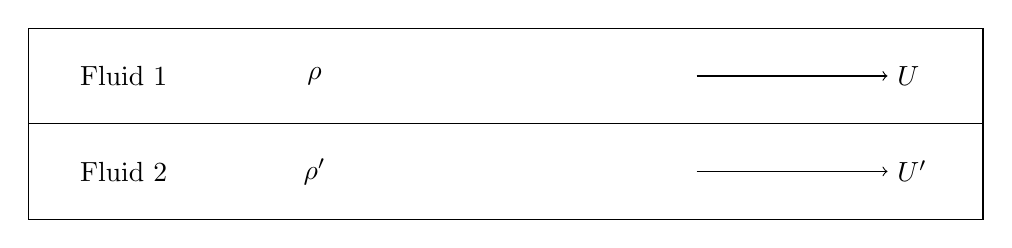
\begin{tikzpicture}[x = \columnwidth/10, y = -\columnwidth/10]
  \draw (0,0) rectangle (10,1);
  \draw (1,0.5) node {Fluid 1};
\draw (3,0.5) node {$\rho$};
  \draw [->] (7,0.5) -- (9,0.5) node [right] {$U$};
  \draw (0,1) rectangle (10,2);
  \draw (1,1.5) node {Fluid 2};
\draw (3,1.5) node {$\rho'$};
  \draw [->] (7,1.5) -- (9,1.5) node [right] {$U'$};
\end{tikzpicture}

From equation (\ref{eq:38}) we have
\begin{equation}
  \label{eq:48}
  \nabla F(t) = \nabla \qty( -\pdv{\phi}{t} + \half \vec{v}^2 + \frac{p}{\rho} + \psi) = 0
\end{equation}
So $F(t)$ is constant throughout space, and $\psi = gz$ is the
gravitational potential. We introduce a perturbation, $\xi(x,z,t)$,
and using equation (\ref{eq:48}) conclude that the pressure on either
side is
\begin{subequations}
  \begin{align}
    p' &= - \rho' \qty( - \pdv{\phi}{t} + \half \vec{v}'^2 + gz ) + \text{constant} \\
p &= - \rho \qty(\pdv{\phi}{t} + \half \vec{v}^2 + gz ) + \text{constant}
  \end{align}
\end{subequations}
At the interface these must be equal, so at $z=\xi$,
\begin{equation}
  \label{eq:49}
   \rho' \qty( - \pdv{\phi}{t} + \half \vec{v}'^2 + g \xi ) = \rho \qty(\pdv{\phi}{t} + \half \vec{v}^2 + g\xi ) + K(t)
\end{equation}
for spatial constant $K$. If we impose a boundary condition that at
all times the perturbation tends to $0$ as $z$ increases then $K$ is
constant in time too.

To find $K$ consider the unperturbed case with $\xi=0$, so
\begin{align*}
  \phi&=0 & \phi' &= 0 \\
v &= U & v' &= U'
\end{align*}
again, as pressures balance at the interface,
\begin{equation}
  \label{eq:50}
  K = \rho \frac{U^2}{2} - \rho' \frac{U'^2}{2}
\end{equation}
so, for a small $\xi$, and given that $\vec{v} = U \vec{e}_x - \nabla \phi$,
\begin{subequations}
  \begin{align}
    v^2 &= (U \vec{e}_x - \nabla \phi)^2 = U^2 - 2 U \pdv{\phi}{x} + \cdots \\
v'^2 &= (U' \vec{e}_x - \nabla \phi)^2 = U'^2 - 2 U' \pdv{\phi'}{x} + \cdots
  \end{align}
\end{subequations}
Hence
\begin{equation}
  \label{eq:51}
  \rho \qty(-\pdv{\phi}{t} - U \pdv{\phi}{x}+ g \xi) = \rho' \qty(- \pdv{\phi'}{t} - U' \pdv{\phi'}{x} + g \xi)
\end{equation}
Introducing small perturbations,
\begin{subequations}
  \begin{align}
    \xi &= A \exp( - i \omega t + i k x) \\
  \phi &= C \exp( - i \omega t + i k x + kz) \\
  \phi' &= C' \exp( - i \omega t + i k x - kz) 
  \end{align}
\end{subequations}
If $\phi$ and $\phi'$ are perturbations on the velocity potential,
then the total velocity potential can be written by redefining the
potential,
\begin{subequations}
  \begin{align}
    -Ux +\phi &\to \phi \\
-U' x + \phi' &\to \phi'
  \end{align}
\end{subequations}
Then the Lagrangian derivative of $\xi$ is
\begin{equation}
  \label{eq:52}
  \dv{\xi}{t} = v_z = - \pdv{\phi}{z}
\end{equation}
So
\begin{subequations}
  Below the surface
  \begin{equation}
    \label{eq:53}
    - \pdv{\phi}{z} = \pdv{\xi}{t}+U \pdv{\xi}{x}
  \end{equation}
and above it
\begin{equation}
  \label{eq:54}
  - \pdv{\phi'}{z} = \pdv{\xi}{t} + U' \pdv{\xi}{x}
\end{equation}
\end{subequations}
Substituting the equations for $\xi$, $\phi$, and $\phi'$ we get
\begin{subequations}
  \begin{align}
    iA (-\omega +kU) &= -k C \\
iA (-\omega +kU') &= k C' \\
\rho(-iC (-\omega +kU) +gA) &= \rho'(-iC'(-\omega+kU')+gA)
  \end{align}
\end{subequations}
These can be solved for $\omega(k)$, and
\begin{equation}
  \label{eq:55}
  \rho (-\omega + kU)^2 + \rho' (-\omega + kU')^2 = kg(\rho-\rho')
\end{equation}
so
\begin{fequation}[Two-fluid Interface Dispersion Relation]
  \label{eq:two-fluid}
  \frac{\omega(k)}{k} = \frac{\rho U + \rho'U'}{\rho+\rho'} \pm \qty( \frac{g}{k} \frac{\rho-\rho'}{\rho+\rho'} - \frac{\rho \rho'(U-U')^2}{(\rho+\rho')^2} )^{\half}
\end{fequation}

There are now a number of ways of producing instabilities. In summary
\begin{description}
\item[Rayleigh-Taylor] Fluids at rest, when $\rho < \rho'$
\item[Kelvin-Helmholtz] When $\rho \rho' (U-U')^2 > \frac{g}{k} (\rho^2 - \rho'^2)$
\item[Jeans Instability] When $\omega^2 = c~S^2 (k^2 - k~J^2)$
\end{description}

\subsection{Rayleigh-Taylor instability}
\label{sec:rayl-tayl-inst}

Let the two fluids be at rest, so $U=U'=0$, but assume that the denser
fluid is above the lighter one, so $\rho<\rho'$. This is intuitively
an unstable equilibrium. The dispersion relation has a solution
\begin{equation}
  \label{eq:57}
  \frac{\omega(k)}{k} = \pm \sqrt{\frac{g}{k} \frac{\rho-\rho'}{\rho+\rho'}}
\end{equation}
for the situation $\rho<\rho'$ we find there is an imaginary part of
$\omega/k$, so
\[ \xi = A \exp(-i \omega t + i k x) = A e^{( \Im(\omega) t) }e^{ -i
\Re(\omega) t + i k x} \] When $\Im(\omega)>0$ the small perturbation
grows exponentially in time, producing an instability.

\subsection{Kelvin-Helmholtz instability}
\label{sec:kelv-inst}

Consider the case where $U \neq U' \neq 0$, but $\rho > \rho'$. The
square-root of equation (\ref{eq:two-fluid}), and so the frequency
$\omega$ is complex, so we get an instability if
\begin{equation}
  \label{eq:58}
  \rho \rho' (U-U')^2 > \frac{g}{k} (\rho^2-\rho'^2)
\end{equation}
Thus
\begin{equation}
  \label{eq:59}
  k > g \frac{\rho^2 - \rho'^2}{\rho \rho' (U - U')^2} 
\end{equation}
is the condition for the instability to occur; as a result it is
possible to avoid the instability at sufficiently long wavelengths.

\subsection{Acoustic waves}
\label{sec:acoustic-waves}

Consider a homogeneous perfect gas with density $\rho_0$ and pressure
$p_0$, then the hydrodynamic equations for a compressible ($\nabla
\vec{v} \neq 0$) without gravity become
\begin{subequations}
  \begin{align}
\label{eq:61}
    \pdv{\rho}{t} + \nabla(\rho \vec{v}) &= 0 \\
\label{eq:62}
\rho \qty( \pdv{t} + (\vec{v} \vdot \nabla) ) \vec{v} &= - \nabla p
  \end{align}
\end{subequations}
Now, we introduce a pressure perturbation, $p = p_0 + \delta p$ and a
density perturbation $\rho = \rho_0 + \delta \rho$. The perturbations
generate a velocity field $\vec{v} = \delta \vec{v}$ assuming there
are no flows in the gas initially, so $\vec{v}_0 = 0$. Substituting
these into the continuity equation
\begin{equation}
  \label{eq:60}
  \pdv{t}(\rho_0 + \delta \rho) + \nabla \qty( (\rho_0 + \delta \rho) \delta \vec{v}) = 0
\end{equation}
Then, as $\rho_0$ is constant,
\[ \pdv{\delta p}{t} + \rho_0 \nabla \vdot \delta \vec{v} = 0 \] with
only the linear components retained. Then, from Euler's equation (\ref{eq:62})
\[ (\rho_0 + \delta \rho) \qty( \pdv{t} + (\delta \vec{v} \vdot \nabla)) \delta \vec{v} = - \nabla (p_0 + \delta p) \]
Which linearises to
\begin{equation}
  \label{eq:64}
  \rho_0 \pdv{\delta \vec{v}}{t} = - \nabla \delta p
\end{equation}
Solving the linear continuity and Euler equations requires a relation
between $\delta p$ and $\delta \rho$, which is the equation of
state. In a perfect gas the motion is adiabatic, so
\begin{equation}
  \label{eq:65}
  \delta p = \eval{\pdv{p}{\rho}}_{p = p_0} \delta \rho
\end{equation}
Using this relation between the density and pressure perturbations the
system of equations becomes
\begin{subequations}
  \begin{align}
    \pdv{\delta \rho}{t} + \rho_0 \nabla \vdot \delta \vec{v} &= 0 \\
\pdv{\delta \vec{v}}{t} &= - \frac{1}{\rho_0} \eval{\pdv{p}{\rho}}_{p=p_0} \nabla \delta \rho
  \end{align}
\end{subequations}
Differentiating the second equation with respect to time, and
substituting from the first equation,
\[ \pdv[2]{\delta \vec{v}}{t} = - \frac{1}{\rho_0} \eval{\pdv{p}{\rho}}_{p=p_0} \nabla \pdv{\delta \rho}{t} = \eval{\pdv{p}{\rho}}_{p=p_0} \Lap \delta \vec{v} \]
Thus we obtain a wave equation for $\delta \vec{v}$, 
\begin{equation}
  \label{eq:66}
  \pdv[2]{\delta \vec{v}}{t} - c~s^2 \Lap \delta \vec{v} = 0
\end{equation}
With $c~s$ the sound speed. The adiabatic gas law,
\[ p = p_0 \qty( \frac{\rho}{\rho_0} )^{\gamma} \] the sound speed can
be expressed in terms of the unperturbed fluid, so
\[ c~s^2 = \eval{\pdv{p}{\rho}}_{p=p_0} = \gamma \frac{p_0}{\rho_0} = \gamma \frac{k~B T}{m} \]
for $k~B$ the Boltzmann constant, since $p = \rho k~B T /m$.

Now, for the dispersion relation, consider a plane-wave perturbation,
$\delta \vec{v} \propto \exp(-i \omega t + i \vec{k} \vdot \vec{r})$; substituting this into the wave equation,
\begin{equation}
  \label{eq:67}
  \omega^2 = c~s^2 k^2
\end{equation}

\subsection{Jeans instability}
\label{sec:jeans-instability}

In the case that a fluid is self-gravitating, we can investigate a
perturbation of the gravitational potential. Let $\psi = \psi_0 +
\delta \psi$ be a perturbed gravitational potential, then
\[ - \nabla p_0 - \rho_0 \nabla \psi_0 = 0 \] with
\[ \Lap \psi_0 = 4 \pi G \rho_0 \] For an infinite gas there are no
nn-trivial uniform solutions, and for $\psi_0$ constant we find
$\rho_0 = 0$. However, if we assume there is an additional force
producing an equilibrium, perturbing and linearising the continuity
equation results in
\[ \pdv{\delta \rho}{t} + \rho_0 \nabla \delta \vec{v} = 0 \]
Linearising the Euler equation, then subtracting the equilibrium
equation, $\nabla p_0 = - \rho_0 \nabla \psi_0$,
\[ \rho_0 \pdv{\delta \vec{v}}{t} = -c~s^2 \nabla \delta \rho - \rho_0 \nabla \delta \psi \]
Similarly, subtracting the equilibrium force from the Poisson equation,
\begin{equation}
  \label{eq:68}
  \Lap \delta \psi = 4 \pi G \delta \rho
\end{equation}
Letting the perturbations vary as $\exp(-i \omega t + i \vec{k} \vdot
\vec{r})$ we have the system of linear equations
\begin{subequations}
  \begin{align}
    - \omega \delta \rho + \rho_0 \vec{k} \delta \vec{v} &= 0 \\
- \rho_0 \omega \delta \vec{v} &= - c~s^2 \vec{k} \delta \rho - \rho_0 \vec{k} \delta \psi \\
- k^2 \delta \psi &= 4 \pi G \delta \rho
  \end{align}
\end{subequations}
Combining these, and eliminating the $\delta$-terms, we find
\begin{equation}
  \label{eq:69}
  \omega^2 = c~s^2 k^2 - 4 \pi G \rho_0 = c~s^2 (k^2 - k~J^2)
\end{equation}
for $k~J^2 = 4 \pi G \rho_0 / c~s^2$. For all $k < k~J$ we find
$\omega$ must be imaginary, producing an instability, the Jeans
instability. Hence a perturbation with a wavelength
\[ \lambda > \lambda~G = \frac{2 \pi}{k~J} = c~s \sqrt{\frac{\pi}{G
    \rho_0}} \] has enough self-gravity to overpower the excess
pressure. The corresponding \emph{Jeans mass} is the mass of a
spherical volume with a diameter of one Jeans wavelength,
\begin{equation}
  \label{eq:70}
  M~J = \frac{4 \pi}{3} \rho_0 \qty( \frac{\lambda~J}{2})^3 = \frac{\pi^{5/2}}{6} \frac{c~s^3}{G^{3/2} \rho_0^{1/2}}
\end{equation}
Given that $c~s^2 = \gamma k~B T/m$,
\begin{equation}
  \label{eq:71}
  \lambda~J = \sqrt{\frac{\gamma \pi k~B T}{m G \rho_0}}
\end{equation}
and
\begin{equation}
  \label{eq:72}
  M~J = \frac{\pi^{5/2}}{6 \rho_0^{1/2}} \qty( \frac{\gamma k~B T}{m G} )^{3/2}
\end{equation}

\section{Shockwaves}
\label{sec:shockwaves}

When the amplitude of a wave is not small the procedure of splitting
the perturbed and unperturbed fluid variables ceases to be
valid. Consider a one-dimensional density wave with $\vec{v} =
(v,0,0)$, so the Euler equation is
\begin{equation}
  \label{eq:56}
  \pdv{v}{t} + v \pdv{v}{x} = - \frac{1}{\rho} \pdv{p}{x}
\end{equation}

We need the other hydrodynamic equations to make any headway, but
simplifying things slightly,
\begin{equation*}
  \pdv{v}{t} + v \pdv{v}{x} = 0
\end{equation*}
and considering its integral curves, $\dv*{x}{t} = v$ in the
$(x,t)$-plane we find the total derivative of $v$ along one of these
curves to be
\[ \dv{t} v(x(t),t) = \pdv{v}{t} + \pdv{v}{x} \dv{x}{t} \]
so along any curve $\dv*{x}{t}=v$ we find $\dv*{v}{t}=0$.

In the simplification of equation (\ref{eq:56}) the solution has the
form \[ v(x,t) = v(x-vt) \] which says that the larger the velocity
$v$ the larger the wave amplitude. As a result of the non-linear
component, $(\vec{v} \vdot \nabla) \vec{v}$ in Euler's equation the
wave-front is steepened, forming a shock-front.

Now consider the pressure term, $\nabla p$,
\[ \pdv{v}{t} + v \pdv{v}{x} = - \frac{1}{\rho} \pdv{p}{x} \]
and the one-dimensional continuity equation,
\[ \pdv{\rho}{t} + \pdv{v \rho}{x} = 0 \] These two equations can be
re-written in a more symmetric form,  with $p = p(\rho)$, and
$c~s^2(\rho) = \pdv*{p}{\rho}$ and $\chi = \log(\rho)$

\begin{subequations}
  \begin{align}
    \pdv{v}{t} + v \pdv{v}{x} &= - c~s^2 \pdv{\chi}{x} \\ 
\pdv{\chi}{t} + v \pdv{\chi}{x} &= - \pdv{v}{x}
  \end{align}
\end{subequations}
Multiplying through the continuity equation by $c~s(\rho)$ we can
combine these
\begin{equation}
  \label{eq:63}
  \pdv{v}{t} + (v+c~s) \pdv{v}{x} = - c~s \qty( \pdv{\chi}{t} + (v + c~s) \pdv{\chi}{x})
\end{equation}
So the disturbance travels at a speed $(v+c~s)$. If the amplitude of
the wave is small $v$ can be neglected, but density fluctuations
propagate with a constant speed $c~s$. When the amplitude is larger
the velocity $v$ becomes important, and the solution becomes
non-linear. The characteristic velocities
\[ \dv{x}{t} = v \pm c~s \]
give the trajectories of the fluid elements along which the quantities 
\[ v \pm \int \frac{c~s}{\rho} \dd{\rho} \] are conserved. These are
Riemann invariants.

\section{Rankine-Hugoniot conditions}
\label{sec:jump-cond-envel}

A shockwave is a thin region of the fluid where dynamic variables
change rapidly. Consider the discontinuity across which various
hydrodynamic variables ``jump''.
% \begin{tikzpicture}[x = \columnwidth/10, y=-\columnwidth/10]
%   \draw (5,0) -- (5,2);
% \draw (4,1) node {$v_1$};
% \draw [->](0,0.5) -- (4.5,0.5); \draw [->] (0, 1.5) -- (4.5, 1.5);
% \draw (6,1) node {$v_1$};
% \end{tikzpicture}
Consider a shock propagating in a medium with density $\rho_1$ and at
a pressure $p_1$ in the shock rest frame. The one-dimensional
hydrodynamic equations are then, in a conservative form,
\begin{subequations}
  \begin{align}
    \pdv{\rho}{t} + \nabla_x (\rho v) &= 0\\
\pdv{\rho v}{t} + \nabla_x(\rho v^2 + p) &= 0\\
\pdv{E}{t} + \nabla_x ([E+p]v)&=0
  \end{align}
\end{subequations}
For \[E = \rho \epsilon + \frac{\rho v^2}{2} \] the total energy per
unit volume, and the shock propagates in the $x$-direction. We assume
the process to be adiabatic, so $p = \rho^{\gamma}$ for $\gamma$ the
adiabatic index, and so
\[ p = (\gamma-1) \rho \epsilon \]
closes the system.

In steady conditions we expect the mass, momentum, and energy fluxes
to be conserved, and at the shock front discontinuity these must also
be conserved. If the shock propagates into a region at density
$\rho_2$ and with pressure $p_2$, then
\begin{align*}
  \rho_1 v_1 &= \rho_2 v_2 \\
\rho_1 v_1^2 + p_1 &= \rho_2 v_2^2 + p_2 \\
\half v_1^2 + \frac{\gamma p_1}{(\gamma-1)\rho_1} &= \half v_2^2 + \frac{\gamma p_2}{(\gamma-1) \rho_2}
\end{align*}
Let us now define the Mach number,
\begin{fequation}[Mach Number]
  \label{eq:73}
  M = \frac{v}{c~{s}} = \frac{v}{\sqrt{\frac{\gamma p}{\rho}}}
\end{fequation}
which is the ratio of the velocity of propagation to the velocity of
pressure wave (sound) propagation, then we can also define the
compression ratio,
\begin{equation}
  \label{eq:74}
  \frac{\rho_2}{\rho_1} = \frac{(\gamma+1)M_1^2}{2+(\gamma-1)M_1^2}
\end{equation}
Clearly, as $M_1 < 1$ this ratio is less than 1, and the shock
disappears, but when $M_1>1$ the ratio grows with $M_1$, and the shock
front forms. $\rho v$ must be constant, so a stronger compression must
move faster, and so the pressure ratio becomes
\begin{equation}
  \label{eq:75}
  \frac{p_1}{p_2} = \frac{(\gamma+1) - (\gamma-1) \rho_2/\rho_1}{(\gamma+1)\rho_2/\rho_1 - (\gamma-1)}
\end{equation}

The equations which relate the variables before and after the shock front are the Rankine-Hugoniot conditions. The density compression has a limiting value for $M \to \infty$,
\begin{equation}
  \label{eq:76}
  \frac{\rho_2}{\rho_1} \to \frac{\gamma+1}{\gamma-1}
\end{equation}
For a monatomic gas $\gamma = \frac{5}{3}$, so the maximum $\rho_2/\rho_1 = 4$. In a diatomic gas $\gamma \approx 1.4$ so $\rho_2/\rho_1 = 6$.

\section{Supernova remnant expansion}
\label{sec:supern-remn-expans}

The expansion of a supernova remnant evolves in three phases,
\begin{enumerate}
\item Free expansion --- ejecta expands without decelerating, so $r \propto t$
\item Adiabatic (Sedov-Taylor) expansion --- energy is conserved
\item Radiative expansion --- energy is disappated into the interstellar medium
\end{enumerate}

\subsection{The Sedov-Taylor regime}
\label{sec:sedov-taylor-regime}

A sudden explosion of gas in a localised region produces a spherical
shockwave which spreads outwards. The Rankine-Hugoniot conditions must
hold across the shock front,so consider the energy $E$, which is
released suddently into a pressureless medium with density $\rho_0$
($p_0 \approx 0)$. $\lambda$ is the scale parameter which describes
the size of the blast wave at a time $t$ after the explosion,
\begin{equation}
  \label{eq:77}
  \lambda = \qty( \frac{E t^2}{\rho_0})^{\frac{1}{5}}
\end{equation}
The radius of the shell just evolve in the same way as $\lambda$, so
\begin{equation}
  \label{eq:78}
  r~s(t) = \zeta_0 \qty( \frac{E t^2}{\rho_0})^{\frac{1}{5}}
\end{equation}
The velocity evolves as
\begin{equation}
  \label{eq:79}
  v~s(t) = \dv{r~s(t)}{t} = \frac{2}{5} \frac{r~s(t)}{t} = \frac{2}{5} \zeta_0 \qty(\frac{E}{\rho_0 t^3})^{1/5}
\end{equation}
Thus the size of the spherical blast increases as $t^{2/5}$ but the
velocity falls off as $t^{-3/5}$. This is the Taylor-Sedov expansion
for an adiabatic blast wave. A typical supernove ejects around $1
M_{\odot}$ of material at a velocity of
$10^4\,\kilo\meter\,\second^{-1}$, so has an energy $E\sim
10^{44}\,\joule$ assuming the material has a density of
$2\e{-21}\,\kilogram\,\meter^{-3}$. Thus, assuming $\zeta_0=1$,
\begin{subequations}
\begin{equation}
  \label{eq:80}
  r~s (t) \approx 0.3 \qty( \frac{t}{1\,\text{year}} )^{2/5}\,\text{pc}
\end{equation}
\begin{equation}
  \label{eq:81}
  v~s (t) \approx 10^5 \qty(\frac{t}{1\,\text{year}})^{-3/5}\,\kilo\meter\,\second^{-1}
\end{equation}
\end{subequations}
These relations become invalid after around $10^5$ years due to the
cooling of the ejecta, but are a very good approximation for the first
hundred years of expansion.

\section{Particle acceleration by supernovae}
\label{sec:part-accel-supern}

The first cosmic rays were observed in 1902 in a railway tunnel
outside Peebles, Scotland by CTR Wilson, but the first correct
determination that these particles were of cosmic origin was due to V
Hess in 1912, from a $5\,\kilo\meter$ balloon experiment. Since then
indirect measurements of the particles from supernova remnants have
been made through their synchrotron emission in the x-ray regime.

\subsection{Fermi acceleration}
\label{sec:fermi-acceleration}

Consider a relativistic particle reflecting from a moving mirror. If $\vec{v}~s$
is the velocity of the shock structure (which acts as the magnetic mirror) then the change in energy for the particle when reflected, $\Delta E$, is 
\[ \Delta E = - 2E \frac{\vec{v}~s \vdot \vec{v}_{\parallel}}{c^2} \]
For $c$ the speed of light. Assuming an isotropic distribution of
energetic ultra-relativistic particles, we find the energy given to a
particle by the shock is
\[ \frac{\ev{\Delta E}}{E} = \frac{4}{3} \frac{v~s}{c} \] Let us now
assume that there are a large number of shock fronts moving randomly
in all directions. The probability of a head-on collision is
proportional to $v~s + v$, while the probability of overtaking a
collision is proportional to $v- v~s$. Thus
\begin{equation}
  \label{eq:82}
  \ev{ \Delta E} = \frac{v+v~s}{2 v} \Delta E - \frac{v-v~s}{2 v} \Delta E \approx 2 \frac{v~s^2}{c^2} E
\end{equation} 
The average rate of energy gain is
\begin{equation}
  \label{eq:83}
  \dv{E}{t} = \frac{\ev{\Delta E}}{\tau} = 2 \frac{v~s^2}{\tau c^2} E 
\end{equation}
Where $\tau$ is the time between collisions. The energy thus increases
linearly with time,
\begin{equation}
  \label{eq:84}
  E(t) = E_0 \exp( \frac{2 v~s^2}{\tau c^2})
\end{equation}
Let $E = bE_0$ be the average energy of a particle after one
collision, and $P$ the probability that the particle remains within
the acceleration region after one collision. After $k$ collisions
there will be $N = N_0 P^k$ particles with energies above $E =
b^kE_0$, so
\begin{equation}
  \label{eq:85}
  \frac{N}{N_0} = \qty( \frac{E}{E_0} )^{\log(P) / \log(b)}
\end{equation}
so 
\begin{equation}
  \label{eq:86}
  N(E) \propto E^{-1 + \log(P)/\log(b)}
\end{equation}
so the energy distribution of particles has a power-law distribution.

\section{The canonical model of shock acceleration}
\label{sec:canon-model-shock}

Consider the idealised problem of a particle accelerated by a shock
wave with one-dimensional geometry propagating in a medium containing
small-scale magnetic-field inhomogeneities which scatter fast-moving
particles.

Provided that the scattering of fast particles is strong enough to
ensure the isotropy assumption the kinetic equation for relativistic
particles in the stationary diffusion-advection equation is
\begin{equation}
  \label{eq:87}
  \pdv{x} v N = \pdv{x} D \pdv{N}{x} + \frac{1}{3} \pdv{v}{x} \pdv{E} E N
\end{equation}
for $N(E,x)$ the energy distribution of the particles, $v(x)$ the
velocity of the stream, and $D$ the spatial diffusion of the energetic
particles. Thus $E \approx pc$ for $p$ the particle
momentum. Integrating over $x$, with the boundary conditions
\begin{align*}
  N(E)=N_1(E) && v=v_1 && \text{at } x \to - \infty\\
N(E) = N_2(E) && v=v_2 && \text{at } x \to + \infty
\end{align*}
From the integration
\[ v_2 N_2(E) - v_1 N_1(E) + 0 - 0 = \frac{1}{3} (v_2 - v_1) \pdv{E} E N_2(E,x) \]
Then the down-stream particle distribution, $E_2(E)$ is given by the ODE
\begin{equation}
  \label{eq:88}
  N_2(E) = \frac{3}{R-1} E^{-\delta} \int^E_{E_0} N_1(E') E'^{\delta-1} \dd{E'} + C E^{- \delta}
\end{equation}
for $C$ some constant, and $\delta = (R+2)/(R-1)$ the spectral index
of the distribution.  When \[N_1(E) = N_0 \delta(E-E_0) \] from an
injection of particles at energy $E_0$,
\[ N_2(E) \propto E^{-\delta} \] for $E>E_0$. 

In strong shockwaves $R = 3$ to $R=4$, so $\delta = 2$ to
$\delta=2.5$. In cosmic rays the spectrum of ions is an un-broken
power law between $10^9\,\electronvolt$ and $10^6\,\electronvolt$, and
with $\delta \approx 2.6$. As a result supernova shockwaves are one of
the leading candidates to explain the production of these particles.

%%% Variables: 
%%% mode: latex
%%% TeX-master: "../project"
%%% End: 
